%% This template can be used to write a paper for
%% Computer Physics Communications using LaTeX.
%% For authors who want to write a computer program description,
%% an example Program Summary is included that only has to be
%% completed and which will give the correct layout in the
%% preprint and the journal.
%% The `elsarticle' style is used and more information on this style
%% can be found at
%% http://www.elsevier.com/wps/find/authorsview.authors/elsarticle.
%%
%%
\documentclass[preprint,12pt]{elsarticle}

%% Use the option review to obtain double line spacing
%% \documentclass[preprint,review,12pt]{elsarticle}

%% Use the options 1p,twocolumn; 3p; 3p,twocolumn; 5p; or 5p,twocolumn
%% for a journal layout:
%% \documentclass[final,1p,times]{elsarticle}
%% \documentclass[final,1p,times,twocolumn]{elsarticle}
%% \documentclass[final,3p,times]{elsarticle}
%% \documentclass[final,3p,times,twocolumn]{elsarticle}
%% \documentclass[final,5p,times]{elsarticle}
%% \documentclass[final,5p,times,twocolumn]{elsarticle}

%% if you use PostScript figures in your article
%% use the graphics package for simple commands
%% \usepackage{graphics}
%% or use the graphicx package for more complicated commands
\usepackage{graphicx}
%% or use the epsfig package if you prefer to use the old commands
%% \usepackage{epsfig}

%% The amssymb package provides various useful mathematical symbols
\usepackage{amssymb}
%% The amsthm package provides extended theorem environments
%% \usepackage{amsthm}

%% The lineno packages adds line numbers. Start line numbering with
%% \begin{linenumbers}, end it with \end{linenumbers}. Or switch it on
%% for the whole article with \linenumbers after \end{frontmatter}.
%% \usepackage{lineno}

% jons ::: my own packages ::: jons
\usepackage{siunitx}
\usepackage{amsmath}
\usepackage{cancel}
\usepackage{hyperref}

% FloatBarrier
\usepackage{placeins}

\def\eqn#1{Eqn.~(\ref{eqn:#1})}

% \intercal for transpose, \mathbb{R} reals, \mathbb{C} complex numbers
% \usepackage{amssymb} (already provided by template)
% \def\realnumbers{\rm I\!R} % does not generalize to complex numbers...
\def\naturals{\mathbb{N}}
\def\naturalsWithZero{\mathbb{N}_0}
\def\integers{\mathbb{Z}}
\def\realnumbers{\mathbb{R}}
\def\complexnumbers{\mathbb{C}}

% \mathfrak{Re}, \mathfrak{Im}
% \usepackage[frak=esstix]{mathalpha} % on some other systems...
\usepackage[frak=esstix]{mathalfa}
\def\realpart{\mathfrak{Re}}
\def\imagpart{\mathfrak{Im}}

% end ::: my own packages ::: end




%% natbib.sty is loaded by default. However, natbib options can be
%% provided with \biboptions{...} command. Following options are
%% valid:

%%   round  -  round parentheses are used (default)
%%   square -  square brackets are used   [option]
%%   curly  -  curly braces are used      {option}
%%   angle  -  angle brackets are used    <option>
%%   semicolon  -  multiple citations separated by semi-colon
%%   colon  - same as semicolon, an earlier confusion
%%   comma  -  separated by comma
%%   numbers-  selects numerical citations
%%   super  -  numerical citations as superscripts
%%   sort   -  sorts multiple citations according to order in ref. list
%%   sort&compress   -  like sort, but also compresses numerical citations
%%   compress - compresses without sorting
%%
%% \biboptions{comma,round}

% \biboptions{}

%% This list environment is used for the references in the
%% Program Summary
%%
\newcounter{bla}
\newenvironment{refnummer}{%
\list{[\arabic{bla}]}%
{\usecounter{bla}%
 \setlength{\itemindent}{0pt}%
 \setlength{\topsep}{0pt}%
 \setlength{\itemsep}{0pt}%
 \setlength{\labelsep}{2pt}%
 \setlength{\listparindent}{0pt}%
 \settowidth{\labelwidth}{[9]}%
 \setlength{\leftmargin}{\labelwidth}%
 \addtolength{\leftmargin}{\labelsep}%
 \setlength{\rightmargin}{0pt}}}
 {\endlist}

\journal{Computer Physics Communications}

\begin{document}

\begin{frontmatter}

%% Title, authors and addresses

%% use the tnoteref command within \title for footnotes;
%% use the tnotetext command for the associated footnote;
%% use the fnref command within \author or \address for footnotes;
%% use the fntext command for the associated footnote;
%% use the corref command within \author for corresponding author footnotes;
%% use the cortext command for the associated footnote;
%% use the ead command for the email address,
%% and the form \ead[url] for the home page:
%%
%% \title{Title\tnoteref{label1}}
%% \tnotetext[label1]{}
%% \author{Name\corref{cor1}\fnref{label2}}
%% \ead{email address}
%% \ead[url]{home page}
%% \fntext[label2]{}
%% \cortext[cor1]{}
%% \address{Address\fnref{label3}}
%% \fntext[label3]{}

\title{Accurate Biot-Savart Routines with Correct Asymptotic Behavior}

%% use optional labels to link authors explicitly to addresses:
%% \author[label1,label2]{<author name>}
%% \address[label1]{<address>}
%% \address[label2]{<address>}

\author[a]{Jonathan Schilling\corref{author}}
\author[a]{Jakob Svensson}
\author[a]{Udo Höfel}
\author[a]{Joachim Geiger}
% \author[a,b]{Second Author}
% \author[b]{Third Author}

\cortext[author] {Corresponding author.\\\textit{E-mail address:} jonathan.schilling@ipp.mpg.de}
\address[a]{Max-Planck-Institute for Plasma Physics, Wendelsteinstrasse 1, 17489 Greifswald, Germany}
% \address[b]{Second Address}

\begin{abstract}
A set of routines to compute the magnetic vector potential and magnetic field of two types of current carriers is presented.
The (infinitely thin) current carrier types are a straight wire segment and a circular wire loop.
The routines are highly accurate and exhibit the correct asymptotic behavior far away from and close to the current carrier.
A suitable global set of test points is introduced and the methods presented in this work
are tested against results obtained using arbitrary-precision arithmetic on all test points.
The results are accurate to approximately 16 decimal digits of precision when computed using 64 bit floating point arithmetic,
with few exceptions where accuracy drops to 13 digits.
These primitive current carrier types can be used to make up more complex arrangements,
such as a current along a polygon (by means of defining straight wire segments from point to point along the polygon)
and a multi-winding coil with circular cross-section (by positioning circular wire loops at appropriate positions in the coils cross-section).
Reference data is provided along with the code to compute it
for testing the reader's routines against this work.
\end{abstract}

\begin{keyword}
%% keywords here, in the form: keyword \sep keyword
magnetostatics; Biot-Savart; straight wire segment; circular wire loop; magnetic vector potential; magnetic field
\end{keyword}

\end{frontmatter}

%%
%% Start line numbering here if you want
%%
% \linenumbers

% All CPiP articles must contain the following
% PROGRAM SUMMARY.

{\bf PROGRAM SUMMARY}

\begin{small}
\noindent
{\em Program Title:} Accurate Biot-Savart routines with Correct Asymptotic Behavior \\
{\em CPC Library link to program files:} (to be added by Technical Editor) \\
{\em Developer's repository link:} https://github.com/jonathanschilling/abscab \\
{\em Code Ocean capsule:} (to be added by Technical Editor)\\
{\em Licensing provisions:} Apache-2.0 \\
{\em Programming language:} C, Python, Java, Fortran \\
{\em Supplementary material:} Reference output data for all methods described in this article. \\
{\em Nature of problem:}\\
  A common task in computational physics is to compute the magnetic field and magnetic vector potential
  originating from current-carrying wire arrangements in the form of coils and cables.
  These current carriers can be approximated for computational simplicity as infinitely thin filaments
  following the center lines of the real current carrier.
  A current carrier path specified by a list of points along the path
  can be modeled as a set of straight wire segments from point to point along the polygon describing the current carrier geometry.
  Closed circular wire loops appear as well in practise and can be chosen to model, e.g.,
  individual windings in a circular coil.
  Computational methods are thus needed to compute the magnetic field and the magnetic vector potential
  of a single straight wire segment or a single circular wire loop
  in order to model more complex current carrier arrangements
  by superposition of the current carrier primitives. \\
{\em Solution method(approx. 50-250 words):}\\
  Analytical expressions are derived in this work to accurately compute
  the magnetic field and the magnetic vector potential of a straight wire segment
  and a circular wire loop. The expressions consist of several special cases,
  which are switched between depending on the location of the evaluation location
  in the coordinate system of the current carrier primitive.
  This approach allows to select the most accurate formulation
  for a given evaluation location and make explicit use of simplications
  in certain special cases for the sake of simplicity, speed and accuracy.
  Particular attention was paid to make sure that the expressions presented in this work
  obey the correct asymptotic behavior for evaluation locations
  far away from and close to the current carriers. \\
{\em Additional comments including restrictions and unusual features (approx. 50-250 words):}\\
  For most test cases, the full relative accuracy of the floating point
  arithmetic chosen for implementation is retained throughout the computations
  (16 digits of precision in the \texttt{binary64} implementation),
  with few exceptions where accuracy drops by up to 2 digits of precision
  (in the \texttt{binary64} case).
  The provided implementations have not been optimized for speed. \\
\end{small}

%% main text
\section{Introduction}
\label{sec:introduction}
A common task in computational physics is to compute the magnetic field and magnetic vector potential
originating from current-carrying wire arrangements in the form of coils and cables.
These current carriers can be approximated for computational simplicity as infinitely thin filaments
following the center lines of the real current carrier.
A current carrier path specified by a list of points along the path
can be modeled as a set of straight wire segments from point to point along the polygon describing the current carrier geometry.
Closed circular wire loops appear as well in practise and can be chosen to model, e.g.,
individual windings in a circular coil.
Computational methods are thus needed to compute the magnetic field and the magnetic vector potential
of a single straight wire segment or a single circular wire loop
in order to model more complex current carrier arrangements
by superposition of the current carrier primitives.
Analytical expressions are derived in this work to accurately compute
the magnetic field and the magnetic vector potential of a straight wire segment
and a circular wire loop. The expressions consist of several special cases,
which are switched between depending on the location of the evaluation location
in the coordinate system of the current carrier primitive.
This approach allows to select the most accurate formulation
for a given evaluation location and make explicit use of simplications
in certain special cases for the sake of simplicity, speed and accuracy.
Particular attention was paid to make sure that the expressions presented in this work
obey the correct asymptotic behavior for evaluation locations
far away from and close to the current carriers.
For most test cases, the full relative accuracy of the floating point
arithmetic chosen for implementation is retained throughout the computations
(16 digits of precision in the IEEE754 \texttt{binary64}~\cite{ieee754} implementation),
with few exceptions where accuracy drops by up to 2 digits of precision
(in the \texttt{binary64} case).
The provided implementations have not been optimized for speed.

The magnetic field is denoted by $\mathbf{H}$ and
the magnetic flux density $\mathbf{B}$ is then given by $\mathbf{B} = \mu_0 \mu_\mathrm{r} \mathbf{H}$,
where $\mu_0$ is the vacuum magnetic permeability
and $\mu_r$ is the relative permeability, taking material properties into account.
In the field of plasma physics generally and in this work in particular,
these two terms are frequently used synonymously
due to the vanishing magnetic susceptibility $|\chi| \ll 1$ of the plasma,
leading to $\mu_r = 1+\chi \approx 1$.
This is equivalent to considering only vacuum magnetic fields.
Then, magnetic field and magnetic flux density only differ by a factor of $\mu_0$.

\section{Methods}
\label{sec:methods}
In this section, the methods used to compute the magnetic vector potential and the magnetic field
of a straight wire segment and a circular wire loop are established.

\subsection{Straight Wire Segment}
The straight wire segment is handled first.

\subsubsection{Magnetic Vector Potential}
The magnetic vector potential of a straight wire segment
only has component~$A_z$ parallel to the wire that is given by:
\begin{equation}
  A_z(\rho, z) = \frac{\mu_0 I}{4 \pi} \ln \left( \frac{1+\epsilon}{1 - \epsilon} \right)
\end{equation}
with
\begin{align}
  \epsilon =&\, \frac{L}{R_i + R_f} \\
       R_i =&\, \sqrt{\rho^2 + z^2} \\
       R_f =&\, \sqrt{\rho^2 + (1-z)^2} \, .
\end{align}
Here, we use normalized coordinates~$\rho' = \rho/L$ and~$z' = z/L$.
This leads to the following expressions for~$r_i = R_i/L$ and~$r_f = R_f/L$:
\begin{align}
  r_i =&\, \sqrt{{\rho'}^2 +      {z'}^2 } \label{eqn:r_i_default} \\
  r_f =&\, \sqrt{{\rho'}^2 + (1 - {z'})^2} \label{eqn:r_f_default} \\
  \epsilon =&\, \frac{1}{r_i + r_f} \, .
\end{align}
A common prefactor depending on the current~$I$ and~$\mu_0$ is split off:
\begin{equation}
  A_z(\rho, z) = \frac{\mu_0 I}{2 \pi} \tilde{A}_z (\rho', z')
\end{equation}
with
\begin{equation}
  \tilde{A}_z (\rho', z')
  = \frac{1}{2} \ln \left( \frac{1+\epsilon}{1 - \epsilon} \right)
  = \textrm{atanh} (\epsilon) \, .
  \label{eqn:A_z_tilde}
\end{equation}
The rest of this section can thus focus on accurate computation of $\tilde{A}_z (\rho', z')$.

The region close to the wire segment~(``near-field'') is handled by one of the following three formulations.
The parameter~$\epsilon$ approaches a value of~$1$ as the location of the evaluation point comes closer to the wire segment.
Thus, the denominator in \eqn{A_z_tilde} vanishes, leading to a logarithmic singularity in~$\tilde{A}_z$
as the evaluation point~$(\rho', z')$ gets nearer to the wire segment.
It is therefore favorable to formulate the near-field method in terms of~$(1-\epsilon)$:
\begin{align}
  1-\epsilon =&\, 1 - \frac{1}{r_i + r_f} = \frac{r_i + r_f - 1}{r_i + r_f} = \frac{r_i + r_f - 1}{(r_i + r_f - 1) + 1} = \frac{n}{n + 1}
\end{align}
with~$n \equiv r_i + r_f - 1$ approaching~$0$ as the evaluation point approaches the wire segment.
Inserting this formulation for~$1-\epsilon$ into \eqn{A_z_tilde} leads to:
\begin{align}
  \tilde{A}_{z,\mathrm{nf}} (\rho', z')
  =&\, \frac{1}{2}  \left[ \ln\left(2 - (1-\epsilon)        \right) - \ln \left(1 - \epsilon    \right) \right] \nonumber \\
  =&\, \frac{1}{2}  \left[ \ln\left(2 - \frac{n}{n + 1}     \right) - \ln \left(\frac{n}{n + 1} \right) \right] \nonumber \\
  =&\, \frac{1}{2}  \left[ \ln\left(\frac{2(n+1) - n}{n + 1}\right) - \ln \left(\frac{n}{n + 1} \right) \right] \nonumber \\
  =&\, \frac{1}{2}  \left[ \ln\left(n + 2                   \right) \cancel{- \ln\left(n + 1 \right)} - \ln \left( n \right) \cancel{+ \ln \left( n + 1 \right)} \right] \nonumber \\
  =&\, \frac{1}{2}  \left[ \ln\left(n + 2                   \right) - \ln \left( n \right) \right] \, .
\end{align}
The subscript ``nf'' was introduced to indicate that this formulation shall only be used for the near-field.
The method used to compute~$n$ still has to be switched depending to the exact location of the evaluation point:
\begin{equation}
  n = \begin{cases}
        n_{6a} &:\, z' \geq 1 \textrm{ or } \rho'/(1-z') \geq 1 \\
        n_{6b} &:\, z' \geq 0 \textrm{ and } \rho'/z' \leq 1 \\
        n_{6c} &:\, \textrm{else}
      \end{cases} \, .
\end{equation}
% A_6a start
The first special case introduces a nutritious zero~($-z' + z'$) into~$n$:
\begin{equation}
  n_{6a} = (r_i - z') + r_f + (z'-1) \, .
\end{equation}
The first contribution to~$n$ is then computed as follows:
\begin{equation}
  r_i - z' = 2 z' \sin^2(\alpha/2) / \cos(\alpha) \label{eqn:ri_zp}
\end{equation}
with $\alpha = \texttt{atan2}(\rho', z')$.
Additionally, $r_f$ is computed via \eqn{r_f_default} and $(z'-1)$ is computed directly.
% A_6a end
% A_6b start
The second special case is based on the first one and introduces another angle~$\beta$
used to compute~$r_f + (z'-1)$ directly:
\begin{equation}
  (r_f + z' - 1) = 2 (1 - z') \sin^2(\beta/2) / \cos(\beta) \label{eqn:rf_zp_1}
\end{equation}
with~$\beta = \texttt{atan2}(\rho', 1-z')$.
Then, $n$ is computed as:
\begin{equation}
  n_{6b} = (r_i - z') + (r_f + z'-1)
\end{equation}
with $(r_i - z')$ from \eqn{ri_zp} and $(r_f + z' - 1)$ from \eqn{rf_zp_1}.
% A_6b end
% A_6c start
The third special case is formulated slightly differently.
Here, $(r_f-1)$ is formulated as:
\begin{equation}
  r_f - 1 = 2 r_f \sin^2(\beta/2) - z' \label{eqn:rf_1}
\end{equation}
with $\beta$ as in the second special case
and $r_i$ and $r_f$ from \eqn{r_i_default} and \eqn{r_f_default}, respectively.
This leads to:
\begin{equation}
  n_{6c} = r_i + (r_f - 1)
\end{equation}
with $(r_f - 1)$ from \eqn{rf_1}.
% A_6c end
This concludes the methods for the near-field evaluation.
Two further special cases are considered next: $\rho' = 0$ and the combined case ($z'=0$, $z'=1$).
For the case of $\rho'=0$, the following formulation should be used:
\begin{equation}
  \tilde{A}_z (\rho'=0, z')
  = \begin{cases}
      \tilde{A}_2(z')  &:\, z' < 1 \textrm{ or } z' > 2 \\
      \tilde{A}_2b(z') &:\, \textrm{else, except } z' \in [0, 1]
    \end{cases}
\end{equation}
with
\begin{equation}
  \tilde{A}_2(z') = \textrm{atanh}\left( \frac{1}{|z'| + |1 - z'|} \right)
\end{equation}
and
\begin{equation}
  \tilde{A}_2b(z') = \frac{1}{2} \textrm{sgn}(z') \ln \left(\left| \frac{z'}{1-z'} \right| \right) \, .
\end{equation}
The following formulation should be used for the cases $z'=0$ or $z'=1$:
\begin{equation}
  \tilde{A}_z (\rho', z' \in \{0, 1\})
  = \begin{cases}
      \tilde{A}_3(\rho')  &:\, \rho' > 1 \\
      \tilde{A}_bb(\rho') &:\, \textrm{else}
    \end{cases}
\end{equation}
with
\begin{equation}
  \tilde{A}_3(z') = \textrm{atanh}\left( \frac{1}{\rho' + \sqrt{{\rho'}^2 + 1}} \right)
\end{equation}
and
\begin{align}
  \tilde{A}_3b(z') =&\, \frac{1}{2} \ln \left(\frac{\rho' c + 1 + c}{\rho' c + 2 s^2 }\right) \\
  c =&\, \cos(\alpha) = \left[{\rho'}^2 + 1 \right]^{-1/2} \\
  s =&\, \sin(\alpha/2)  \\
 \alpha =&\, \arctan(\rho') \, .
\end{align}
If none of above special cases applies,
the following general formulation is used for the ``far-field'' case:
\begin{equation}
  \tilde{A}_{z,\mathrm{ff}} (\rho', z') = \textrm{atanh}\left( \frac{1}{r_i + r_f} \right)
\end{equation}
with $r_i$ and $r_f$ from \eqn{r_i_default} and \eqn{r_f_default}, respectively.
%
% total assembly of A_z for straight wire segment
%
The overall switching between the methods introduced above is done as follows:
\begin{equation}
  \tilde{A}_z (\rho', z')
  = \begin{cases}
      \tilde{A}_z (\rho'=0, z')             &:\, \rho' = 0 \\
      \tilde{A}_z (\rho', z' \in \{0, 1\})  &:\, z' \in \{0, 1\} \\
      \tilde{A}_{z,\mathrm{nf}} (\rho', z') &:\, z' \in ]-1, 2] \textrm{ and } \rho' < 1 \\
      \tilde{A}_{z,\mathrm{ff}} (\rho', z') &:\, \textrm{else}
    \end{cases} \, .
\end{equation}

\subsubsection{Magnetic Field}
The magnetic field of a straight wire segment
only has a tangential component~$B_\varphi$ around the wire that is given by:
\begin{equation}
  B_\varphi(\rho, z) = \frac{\mu_0 I}{4 \pi} \frac{2 L (R_i + R_f)}{R_f} \frac{1}{\left(R_i + R_f\right)^2 - L^2}
\end{equation}
with~$L$, $R_i$ and $R_f$ as in the previous section.
Again a normalization factor is split off:
\begin{equation}
  B_\varphi(\rho, z) = \frac{\mu_0 I}{4 \pi L} \tilde{B}_\varphi(\rho', z')
\end{equation}
with
\begin{align}
  \tilde{B}_\varphi(\rho', z')
  =&\, \frac{2 L^2(R_i + R_f)}{R_f} \frac{1}{\left(R_i + R_f\right)^2 - L^2} \nonumber \\
  =&\, \left(\frac{r_i}{r_f} + 1\right) \frac{2}{\left(r_i + r_f\right)^2 - 1} \, .
\end{align}
The special case~$\rho'=0$ is handled first:
\begin{equation}
  \tilde{B}_\varphi(\rho'=0, z') = \frac{1}{2} \left( \frac{1}{(1-z')^2} - \frac{1}{z'(1-z')} \right) \, .
\end{equation}
Similarly, a special case for~$z' \in \{0, 1\}$ can be derived:
\begin{equation}
  \tilde{B}_\varphi(\rho', z' \in \{0, 1\}) = \frac{1}{\rho' \sqrt{{\rho'}^2 + (1-z')^2}} \, .
\end{equation}
The next method handles the evaluation locations far away from the loop
as well as a part of the near-field:
\begin{equation}
  \tilde{B}_{\varphi,4} (\rho', z')
  = \left(\frac{r_i}{r_f} + 1\right) \frac{1}{{\rho'}^2 + r_i r_f - z' (z' - 1)} \, .
\end{equation}
For certain evaluation points close to the loop,
the terms~$r_i r_f$ and $-z' (z' - 1)$ in above formula almost cancel each other.
This cancellation introduces a requirement for one more method to compute~$\tilde{B}_\varphi (\rho', z')$:
\begin{equation}
  \tilde{B}_{\varphi, 5} (\rho', z')
  = \frac{r_i / r_f + 1}
         {{\rho'}^2 + z' (1 - z') \frac{2}{\cos(\alpha)} \left( \frac{\sin^2(\beta/2)}{\cos(\beta)} + \sin^2(\alpha/2) \right)}
\end{equation}
with~$\alpha$ and~$\beta$ as introduced for \eqn{ri_zp} and \eqn{rf_zp_1}.
%
% total assembly of B_phi for straight wire segment
%
The overall switching between the methods introduced above is done as follows:
\begin{equation}
  \tilde{B}_\varphi (\rho', z')
  = \begin{cases}
      \tilde{B}_\varphi(\rho'=0, z')             &:\, \rho' = 0 \\
      \tilde{B}_\varphi(\rho', z' \in \{0, 1\})  &:\, z' \in \{0, 1\} \\
      \tilde{B}_{\varphi,4} (\rho', z') &:\, z' \notin ]0,1[ \textrm{ or } \rho' \geq 1 \\
                                   ~    & ~ \textrm{ or } \rho'/(1-z') \geq 1  \\
                                   ~    & ~ \textrm{ or } \rho'/z'   \geq 1 \\
      \tilde{B}_{\varphi,5} (\rho', z') &:\, \textrm{else}
    \end{cases} \, .
\end{equation}







\subsection{Circular Wire Loop}
The circular wire loop is handled next.

\subsubsection{Magnetic Vector Potential}


\subsubsection{Magnetic Field}


\subsection{Transformation to Cartesian Coordinates}
Evaluation of the magnetostatic quantities~$A_\varphi$, $B_\rho$ and $B_z$ happens in cylindrical coordinates~$\rho$ and~$z$.
It is often more convenient to be able to work in Cartesian coordinates.
Figure~\ref{fig:mappingToCartesian} illustrates the setup of a circular wire loop.
\begin{figure}[htbp]
 \centering
 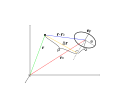
\includegraphics{img/MappingToCartesian.eps}
 \caption{Mapping the components to Cartesian coordinates for an exemplary circular wire loop.
          The loop is centered around its origin~$\mathbf{r}_0$.
          Its normal vector is denoted $\mathbf{n}$ and defines the orientation of the loop.
          The radius of the loop is denoted by~$a$.
          The evaluation location is denoted by~$\mathbf{r}$.}
 \label{fig:mappingToCartesian}
\end{figure}

The $z$-axis of the wire loop's coordinate system is defined by the normal vector~$\mathbf{n}$:
\begin{equation}
  \hat{\mathbf{e}}_z = \frac{\mathbf{n}}{|\mathbf{n}|} \, .
\end{equation}
The $z$ component of the evaluation location is thus obtained as follows:
\begin{equation}
  z = (\mathbf{r} - \mathbf{r}_0) \cdot \hat{\mathbf{e}}_z \, .
\end{equation}
The normalized $z$-coordinate $z'$ is then obtained as:
\begin{equation}
  z' = \frac{z}{a} = \frac{1}{a} (\mathbf{r} - \mathbf{r}_0) \cdot \hat{\mathbf{e}}_z \, .
\end{equation}
For the radial coordinate, first the vector~$\Delta \mathbf{r}$ is formed:
\begin{equation}
  \Delta \mathbf{r} = (\mathbf{r} - \mathbf{r}_0) - z \, \hat{\mathbf{e}}_z
\end{equation}
and the radial coordinate $\rho$ is then obtained by taking $\rho = |\Delta \mathbf{r}|$.
A unit vector in radial direction is formed as follows:
\begin{equation}
  \hat{\mathbf{e}}_\rho = \frac{\Delta \mathbf{r}}{\rho} \, .
\end{equation}
The normalized radial coordinate~$\rho'$ is then obtained as:
\begin{equation}
  \rho' = \frac{\rho}{a} = \frac{1}{a} |(\mathbf{r} - \mathbf{r}_0) - z \, \hat{\mathbf{e}}_z| \, .
\end{equation}
The magnetic field of the circular wire loop consists of two cylindrical components, namely $B_\rho$ and $B_z$.
The Cartesian magnetic field components are then computed as follows:
\begin{equation}
  \mathbf{B}(\mathbf{r}) = B_\rho \hat{\mathbf{e}}_\rho + B_z \hat{\mathbf{e}}_z \, .
\end{equation}
The magnetic vector potential only has a component in angular direction in the coordinate system of the wire loop.
The corresponding unit vector~$\hat{\mathbf{e}}_\varphi$ is then given by
$\hat{\mathbf{e}}_\varphi = \hat{\mathbf{e}}_\rho \times \hat{\mathbf{e}}_z$.
The vector potential of the circular wire loop in thus in Cartesian coordinates:
\begin{equation}
  \mathbf{A}(\mathbf{r}) = A_\varphi \hat{\mathbf{e}}_\varphi \, .
\end{equation}

\subsection{Superposition in multi-filament assemblies}
% PolygonFilament
An infinitely thin polygon filament $P$ is described by a list of $N$ points $\mathbf{x}_i$ with $i=1, ..., N$ in three-dimensional (3D) space and a current $I$.
The $(N-1)$ straight connecting lines between each two consecutive points $\mathbf{x}_i$ and $\mathbf{x}_{i+1}$ are assumed to represent the geometry of a wire which carries the current.
If the first and the last point of the polygon filament coincide, the wire forms a closed loop and $\nabla \cdot \mathbf{j} = 0$ is ensured by construction.

The magnetic vector potential $\mathbf{A}(I, \mathbf{x}_i, \mathbf{x}_{i+1}, \mathbf{x})$ and the magnetic field $\mathbf{B}(I, \mathbf{x}_i, \mathbf{x}_{i+1}, \mathbf{x})$
of the wire segments at a location $\mathbf{x}$ can be computed analytically.
The resulting contributions from each segment are superposed in order to compute the resulting magnetic field from the full length of the wire:
\begin{align}
 \mathbf{A}(\mathbf{x}) & = \sum_{i=1}^{N-1} \mathbf{A}(I, \mathbf{x}_i, \mathbf{x}_{i+1}, \mathbf{x}) \quad \mathrm{and} \\
 \mathbf{B}(\mathbf{x}) & = \sum_{i=1}^{N-1} \mathbf{B}(I, \mathbf{x}_i, \mathbf{x}_{i+1}, \mathbf{x}) \quad .
\end{align}
Computationally robust and efficient expressions for
$\mathbf{A}(I, \mathbf{x}_i, \mathbf{x}_{i+1}, \mathbf{x})$ and
$\mathbf{B}(I, \mathbf{x}_i, \mathbf{x}_{i+1}, \mathbf{x})$
are given in Ref.~\cite{hanson_hirshman_2002}.
The detailed derivation of these expressions is given below.

% multi-winding circular coil

\section{Results}
\label{sec:results}
The results of the verification method introduced in Sec.~\ref{sec:methods_verification}
are presented next.
\subsection{Straight Wire Segment}
First, the results of the verification of the straight wire segment methods are presented.
The normalized vertical component of the magnetic vector potential, $\tilde{A}_z$,
and the normalized tangential component magnetic field, $\tilde{B}_\varphi$, of a straight wire segment
have been evaluated using \eqn{sws_A_z_switchover} and \eqn{sws_B_phi_switchover}, respectively,
on all test points in $T_\mathrm{SWS}$ (see Sec.~\ref{sec:methods_verification}).
The left half of Fig.~(\ref{fig:StraightWireSegment_results}) shows the deviation
between the reference data computed for $\tilde{A}_z$ using \eqn{sws_A_z_ref}
and the results from the \texttt{float64} implementation of \eqn{sws_A_z_switchover}
according to the error metric~\eqn{error_metric}.
The right half of Fig.~(\ref{fig:StraightWireSegment_results}) shows the corresponding deviation
between the reference data computed for $\tilde{B}_\varphi$ using \eqn{sws_B_phi_ref}
and the results from the \texttt{float64} implementation of \eqn{sws_B_phi_switchover}.
\begin{figure}[htbp]
 \centering
 \includegraphics[width=\textwidth]{img/StraightWireSegment_results.pdf}
 \caption{Deviation between the Java implementation of the methods for $\tilde{A}_z$ (left)
          and $\tilde{B}_\varphi$ (right) of a straight wire segment (SWS).
          The left  plot shows the deviation between the Java implementation of \eqn{sws_A_z_switchover}
                         and the arbitray-precision implementation of \eqn{sws_A_z_ref}
          and
          the right plot shows the deviation between the Java implementation of \eqn{sws_B_phi_switchover}
                         and the arbitray-precision implementation of \eqn{sws_B_phi_ref}
          in the error metric given by~\eqn{error_metric}.}
 \label{fig:StraightWireSegment_results}
\end{figure}
It is observed that the relative error is less that $10^{-15}$ for all test points under consideration.

\subsection{Circular Wire Loop}
Next, the results of the verification of the circular wire loop methods are presented.
The normalized tangential component of the magnetic vector potential, $\tilde{A}_\varphi$,
and the normalized radial and vertical components of the magnetic field, $\tilde{B}_\rho$ and $\tilde{B}_z$,
of a circular wire loop have been evaluated using \eqn{A_phi_final}, \eqn{cwl_B_rho_switchover}
and \eqn{cwl_B_z_switchover}, respectively,
on all test points in $T_\mathrm{CWL}$ (see Sec.~\ref{sec:methods_verification}).
Fig.~(\ref{fig:CircularWireLoop_A_phi_Java}) shows the deviation
according to the error metric~\eqn{error_metric}
between the reference data computed for $\tilde{A}_\varphi$ using \eqn{A_phi_ref}
and the results from the \texttt{float64} implementation of \eqn{A_phi_final}.
\begin{figure}[htbp]
 \centering
 \includegraphics[width=0.8\textwidth]{img/CircularWireLoop_A_phi_Java.pdf}
 \caption{Deviation between Java implementation of \eqn{A_phi_final} and \eqn{A_phi_ref}
          for the computation of $\tilde{A}_\varphi$ of a circular wire loop
          in the error metric given by~\eqn{error_metric}.}
 \label{fig:CircularWireLoop_A_phi_Java}
\end{figure}
Fig.~(\ref{fig:CircularWireLoop_B_rho_Java}) shows the deviation
according to the error metric~\eqn{error_metric}
between the reference data computed for $\tilde{B}_\rho$ using \eqn{B_rho_ref}
and the results from the \texttt{float64} implementation of \eqn{cwl_B_rho_switchover}.
\begin{figure}[htbp]
 \centering
 \includegraphics[width=0.8\textwidth]{img/CircularWireLoop_B_rho_Java.pdf}
 \caption{Deviation between Java implementation of \eqn{cwl_B_rho_switchover} and \eqn{B_rho_ref}
          for the computation of $\tilde{B}_\rho$ of a circular wire loop
          in the error metric given by~\eqn{error_metric}.}
 \label{fig:CircularWireLoop_B_rho_Java}
\end{figure}
Fig.~(\ref{fig:CircularWireLoop_B_z_Java}) shows the deviation
according to the error metric~\eqn{error_metric}
between the reference data computed for $\tilde{B}_z$ using \eqn{B_z_ref}
and the results from the \texttt{float64} implementation of \eqn{cwl_B_z_switchover}.
\begin{figure}[htbp]
 \centering
 \includegraphics[width=0.8\textwidth]{img/CircularWireLoop_B_z_Java.pdf}
 \caption{Deviation between Java implementation of \eqn{cwl_B_z_switchover} and \eqn{B_z_ref}
          for the computation of $\tilde{B}_z$ of a circular wire loop
          in the error metric given by~\eqn{error_metric}.}
 \label{fig:CircularWireLoop_B_z_Java}
\end{figure}

\FloatBarrier
\subsection{Further tests}
Furthermore, it was tested if the methods presented in this work
can be used to approximate a circular wire loop
by a polygon along the wire down to numerical accuracy.
The geometry of the setup is depicted in Fig.~(\ref{fig:sketch_McGreivy}).
\begin{figure}[htbp]
 \centering
 \includegraphics[width=0.4\textwidth]{img/sketch_McGreivy.png}
 \caption{Sketch of the test setup for approximating a circular wire loop by a polygon.
          The current along the wire loop (black) is approximated by
          a current along a polygon with vertices either on the loop (red)
          or vertices adjusted slightly outwards (blue).
          The case of $n=5$ vertices used to approximate the loop is shown here.}
 \label{fig:sketch_McGreivy}
\end{figure}
The expected result is that the relative deviation between
the magnetic field at an arbitrary location
from the circular wire loop and from the corresponding polygon approximation
using straight wire segments vanishes down to numerical accuracy
for a sufficiently large number of points~$n$ used to approximate the wire loop.
A second-order correction to the polygon approximation
for a circular wire loop~\cite{mcgreivy_2021} can be used
to improve the approximation.
Here, the vertices of the polygon used to approximate the wire loop
are adjusted slightly outwards.
Figuratively speaking, in the default case (red polygon in Fig.~\ref{fig:sketch_McGreivy})
the polygon segments are always inside the wire loop
and in the adjusted case (blue polygon in Fig.~\ref{fig:sketch_McGreivy}),
the polygon segments have portions both inside and outside the wire loop.
The results of increasing the number of polygon corners
and observing the decay of the relative error between the analytical wire loop
expression and the approximation by the polygon
are shown in Fig.~(\ref{fig:McGreivy_convergence_2}),
where the orange graph with + symbols (``on-loop'') denotes the case of the polygon vertices on the loop
and the cyan graph with x symbols (``McGreivy'') denotes the case of the polygon vertices adjusted towards the outside
according to Ref.~\cite{mcgreivy_2021}.
In those two cases, standard accumulation using the \texttt{+=} operator
was used to sum up the contributions from the individual wire segments.
It is observed that the results approach numerical accuracy.
but then the error grows again if more polygon vertices are used for the approximation.
This can be explained by considering that the more vertices are used,
the smaller the relative contributions from each individual segment to the total approximation get.
If standard accumulation of the results is used, at some number of polygon corners
it happens that the remaining contributions are getting smaller than the machine precision epsilon
of the current approximation result, thereby effectively ignoring the remaining contributions.
Second-order iterative Kahan-Babuska summation~\cite{klein_2006} had to be used
to circumvent this and achive convergence down to numerical accuracy.
This is shown by the red and blue graphs in Fig.~(\ref{fig:McGreivy_convergence_2}),
where the relative deviation from the reference data does not grow
as the number of polygon corners is increased beyond the threshold for an accurate approximation.
\begin{figure}[htbp]
 \centering
 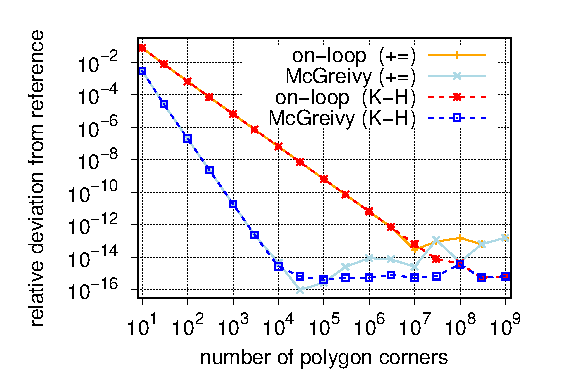
\includegraphics[width=0.8\textwidth]{img/McGreivy_convergence_2.eps}
 \caption{Convergence of the polygon approximation towards the analytical result for the magnetic field of a circular wire loop.
          The vertices of the polygon used to approximate the wire loop have been put on the wire loop (``on-loop'')
          as well as adjusted slightly outwards of the loop according to Ref.~\cite{mcgreivy_2021} (``McGreivy'').
          Standard accumulation using the \texttt{+=} operator (``+='') has been used for the first two graphs (orange and cyan).
          The second two graphs (red and blue) show the results when the accumulation of the individual contributions
          is performed using compensated Kahan-Babushka summation~\cite{klein_2006} (``K-B'')).}
 \label{fig:McGreivy_convergence_2}
\end{figure}

\section{Discussion}
\label{sec:discussion}
Accurate methods have been presented in this work
to compute the magnetic vector potential~$\mathbf{A}$
and the vacuum magnetic field~$\mathbf{B}$
of filamentary current carriers
in the form of a straight wire segment
and a circular wire loop.
Particular attention was paid to make sure that the implemented formulas
are capable of achieving nearly full precision of the floating-point arithmetic
in which they are implemented.
%
The methods for the straight wire segment
achieve 15 out of 16 digits of precision for both
the magnetic vector potential and the magnetic field
in the \texttt{binary64} implementation.
%
The methods for the circular wire loop
achieve 15 digits of precision for the magnetic vector potential
and for the magnetic field far away from the wire loop.
Close to the wire loop, accuracy of the magnetic field methods
drops to 14 digits of precision.
%
The reference data was computed using arbitrary-precision arithmetic
in two very different implementations (namely the open source \texttt{mpmath} Python package
and the commercial Mathematica software) and verified to be sufficiently accurate
for testing the \texttt{binary64} implementations.
This reference data is provided along with this article
to allow the readers to test their own routines.
%
An application is presented where these methods
are used to approximate the magnetic field of a circular current loop
by using a current along a polygon aligned with the shape of the wire loop.
It is demonstrated that the approximation converges to the analytical result
of the wire loop down to machine precision and remains there
for further increases in the number of vertices of the approximating polygon.
This further demonstrates the robustness of the methods presented in this work.
It was found that compensated summation techniques were required
in order to correctly accumulate the superposition of a large number
of individual polygon segments.
The selected second-order Kahan-Babushka summation is therefore used by default in the reference implementation.
%
The asymptotic behaviour of the formulas
when evaluating~$\mathbf{A}$ and~$\mathbf{B}$ close to the current carrier
and far away from it is verified to produce the correct results.
%
The free-boundary part of the Variational Moments Equilibrium Code (VMEC)~\cite{hirshman_1986}
uses interpolation of the vacuum magnetic field produced by the confinement coils
of a Stellarator device~\cite{spitzer_1958}.
It is frequently the case that coils overlap with the region
in which the cached interpolation table is computed for further use.
During iterations of VMEC, it can happen that this way
field values close to the coils enter the computation
and it is deemed beneficary for the robustness of the computation
if those values attain the correct asymptotic values.

\section{Outlook}
\label{sec:outlook}



\section{Acknowledgments}
\label{sec:acknowledgments}
We gratefully acknowledge useful discussions with
S.~Hudson, C.~Zhu, J.~Schmitt, S.~Lazerson and M.~Cianciosa.

This work has been carried out within the framework of the EUROfusion Consortium,
funded by the European Union via the Euratom Research and Training Programme (Grant Agreement No 101052200 - EUROfusion).
Views and opinions expressed are however those of the author(s) only
and do not necessarily reflect those of the European Union or the European Commission.
Neither the European Union nor the European Commission can be held responsible for them.


%% The Appendices part is started with the command \appendix;
%% appendix sections are then done as normal sections
\appendix

%% \section{}
%% \label{}

\section{Derivation of General Formulations}
\label{apx:derivation_of_general_formulations}
The derivations of the starting point formulas presented in Sec.~\ref{sec:methods} are given here.

\subsection{Straight Wire Segment}
The following geometric quantities with $\mathbf{x}_f \equiv \mathbf{x}_{i+1}$ are defined to ease the rest of the derivation:
\begin{align}
 L                   & \equiv | \mathbf{x}_f - \mathbf{x}_i | \, , \\
 \hat{\mathbf{e}}    & \equiv \left(\mathbf{x}_f - \mathbf{x}_i\right) / L \, , \\
 \mathbf{R}_i        & \equiv \mathbf{x} - \mathbf{x}_i \, , \\
 \mathbf{R}_f        & \equiv \mathbf{x} - \mathbf{x}_f \, , \\
 R_i                 & \equiv | \mathbf{R}_i | = | \mathbf{x} - \mathbf{x}_i | \, , \\
 R_f                 & \equiv | \mathbf{R}_f | = | \mathbf{x} - \mathbf{x}_f | \, , \\
 R_{i ||}            & \equiv \hat{\mathbf{e}} \cdot \mathbf{R}_i \, , \\
 R_{f ||}            & \equiv \hat{\mathbf{e}} \cdot \mathbf{R}_f \, , \\
 \mathbf{R}_\perp    & \equiv \mathbf{R}_i - R_{i ||} \hat{\mathbf{e}} \, , \\
 R_\perp             & \equiv | \mathbf{R}_\perp | \quad \mathrm{and} \\
 \mathbf{c}(\lambda) & \equiv \mathbf{x}_i + \lambda \left(\mathbf{x}_f - \mathbf{x}_i\right) \quad \mathrm{for} \quad 0 \leq \lambda \leq 1 \, .
\end{align}
The following relations are also needed:
\begin{align}
       L             & = R_{i ||} - R_{f ||} \\
       R_i^2 - R_f^2 & = L \left( R_{i ||} + R_{f ||} \right) \\
\Rightarrow R_{i ||} & = \frac{R_i^2 - R_f^2}{2 L} + \frac{L}{2} \\
\Rightarrow R_{f ||} & = \frac{R_i^2 - R_f^2}{2 L} - \frac{L}{2}
\end{align}

\subsubsection{Magnetic Vector Potential}
The law of Biot and Savart for the magnetic vector potential of a current density distribution $\mathbf{j}(\mathbf{x})$ is as follows~\cite{jackson}:
\begin{equation}
 \mathbf{A}(\mathbf{x}) = \frac{\mu_0}{4 \pi} \int \frac{\mathbf{j}(\mathbf{x}')}{|\mathbf{x} - \mathbf{x}'|} \mathrm{d}\mathbf{x}' \, .
\end{equation}
The parametrization of points on the line segment $\mathbf{c}(\lambda)$ can be used to apply this to the given geometry of a wire segment:
\begin{align}
 \mathbf{A}(\mathbf{x}) & = \frac{\mu_0 I}{4 \pi} L \hat{\mathbf{e}} \int\limits_0^1 \frac{\mathrm{d}\lambda}{|\mathbf{x} - \mathbf{c}(\lambda)|} \\
        ~               & = \frac{\mu_0 I}{4 \pi} L \hat{\mathbf{e}} \int\limits_0^1 \frac{\mathrm{d}\lambda}{|\mathbf{x} - \mathbf{x}_i - \lambda L \hat{\mathbf{e}}|} \, .
\end{align}
A little bit of geometric intuition is needed to simplify the denominator of the integral:
\begin{align}
 \mathbf{x} - \mathbf{x}_i - \lambda L \hat{\mathbf{e}}
   & = \mathbf{R}_i - \lambda L \hat{\mathbf{e}} \\
 ~ & = \mathbf{R}_i - R_{i ||} \hat{\mathbf{e}} + R_{i ||} \hat{\mathbf{e}} - \lambda L \hat{\mathbf{e}} \\
 ~ & = \mathbf{R}_i - R_{i ||} \hat{\mathbf{e}} + \left( R_{i ||} - \lambda L \right) \hat{\mathbf{e}} \\
 ~ & = \mathbf{R}_\perp + \left( R_{i ||} - \lambda L \right) \hat{\mathbf{e}} \, .
\end{align}
Note that, in particular, $\mathbf{R}_\perp \perp \hat{\mathbf{e}}$ and thus (since $|\hat{\mathbf{e}}|$ = 1) due to Pythagoras:
\begin{equation}
 | \mathbf{x} - \mathbf{x}_i - \lambda L \hat{\mathbf{e}} |^2 = R_\perp^2 + \left( R_{i ||} - \lambda L \right)^2
\end{equation}
and finally with $R_\perp^2 = R_i^2 - R_{i ||}^2$ (also due to Pythagoras):
\begin{align}
 | \mathbf{x} - \mathbf{x}_i - \lambda L \hat{\mathbf{e}} |^2
   & = R_i^2 - R_{i ||}^2 + R_{i ||}^2 - 2 \lambda L R_{i ||} + \lambda^2 L^2 \\
 ~ & = R_i^2 - 2 \lambda L R_{i ||} + \lambda^2 L^2 \, .
\end{align}
It follows:
\begin{equation}
 \mathbf{A}(\mathbf{x})
 = \frac{\mu_0 I}{4 \pi} L \hat{\mathbf{e}} \int\limits_0^1 \frac{\mathrm{d}\lambda}{\sqrt{R_i^2 - 2 \lambda L R_{i ||} + \lambda^2 L^2}} \, . \label{eqn:A_integral}
\end{equation}
For $X = a x^2 + b x + c$ with $a>0$ the following relation holds~\cite{bronstein}:
\begin{equation}
 \int \frac{\mathrm{d}x}{\sqrt{X}} = \frac{1}{\sqrt{a}} \log \left( 2 \sqrt{a X} + 2 a x + b \right) \, .
\end{equation}
Here, $x = \lambda$, $a = L^2$, $b=-2 L R_{i ||}$ and $c=R_i^2$.
The corresponding antiderivative of the integrand in \eqn{A_integral} is:
\begin{align}
 \int&\frac{\mathrm{d}\lambda}{\sqrt{R_i^2 - 2 \lambda L R_{i ||} + \lambda^2 L^2}} \nonumber \\
 =&\, \frac{1}{L} \log \left( 2 \sqrt{L^2\left( L^2 \lambda^2 - 2 L R_{i ||} \lambda + R_i^2 \right)} + 2 L^2 \lambda - 2 L R_{i ||} \right) \, .
\end{align}
The definite integral in \eqn{A_integral} is therefore solved by the following expression:
\begin{align}
 ~ & \int\limits_0^1 \frac{\mathrm{d}\lambda}{\sqrt{R_i^2 - 2 \lambda L R_{i ||} + \lambda^2 L^2}} \\
 = & \frac{1}{L} \Biggl[\phantom{-}\, \log \left( 2 \sqrt{L^2\left( L^2 - 2 L R_{i ||} + R_i^2 \right)} + 2 L^2 - 2 L R_{i ||} \right) \nonumber \\
 ~ & \phantom{\frac{1}{L} \Biggl[} - \log \left( 2 \sqrt{L^2 R_i^2 } - 2 L R_{i ||} \right) \Biggr] \\
 = & \frac{1}{L} \log \left( \frac{ \bcancel{2 L} \sqrt{L^2 - 2 L R_{i ||} + R_i^2} + \bcancel{2} L^{\bcancel{2}} - \bcancel{2 L} R_{i ||} }{ \bcancel{2 L} R_i - \bcancel{2 L} R_{i ||} } \right)
\end{align}
Note that
\begin{align}
                             L^2 & = L (R_{i ||} - R_{f ||} ) \\
                              ~  & = L R_{i ||} - L R_{f ||} \\
\Rightarrow -2 L R_{i ||} + L^2  & = - \bcancel{2} L R_{i ||}  + \bcancel{L R_{i ||}} - L R_{f ||} \\
                              ~  & = -L (R_{i ||} + R_{f ||} ) \\
                              ~  & = R_f^2 - R_i^2 \\
\Rightarrow                R_f^2 & = R_i^2 -2 L R_{i ||} + L^2 \, .
\end{align}
Therefore:
\begin{equation}
 \int\limits_0^1 \frac{\mathrm{d}\lambda}{\sqrt{R_i^2 - 2 \lambda L R_{i ||} + \lambda^2 L^2}}
 = \frac{1}{L} \log \left( \frac{ R_f - R_{f ||} }{ R_i - R_{i  \,\mathrm{d}\varphi||} } \right) \, .
\end{equation}
Inserting this into \eqn{A_integral} leads to the first intermediate result:
\begin{equation}
   \mathbf{A}(\mathbf{x})
 = \frac{\mu_0 I}{4 \pi} \bcancel{L} \bcancel{\frac{1}{L}} \log \left( \frac{ R_f - R_{f ||} }{ R_i - R_{i ||} } \right) \hat{\mathbf{e}}
 = \frac{\mu_0 I}{4 \pi}                                   \log \left( \frac{ R_f - R_{f ||} }{ R_i - R_{i ||} } \right) \hat{\mathbf{e}} \, . \label{eqn:A_first}
\end{equation}
However, if the point $\mathbf{x}$ is located on the line extension of the wire segment, $R_i = R_{i ||}$ and $R_f = R_{f ||}$,
which leads to a $0/0$ division if this formula is directly evaluated.
The solution is to cancel the singular term $(L + R_f - R_i)$, which is also zero for points on the line extension of the wire segment,
in the numerator and the denominator of \eqn{A_first}.
A second look resolves this:
\begin{align}
\frac{ R_f - R_{f ||} }{ R_i - R_{i ||} }
 = & \frac{ 2 L \left( R_f - R_{f ||} \right) }{ 2 L \left( R_i - R_{i ||} \right) }
 =   \frac{ 2 L R_f - 2 L \left( \frac{R_i^2 - R_f^2}{2 L} - \frac{L}{2} \right) }{ 2 L R_i - 2 L \left( \frac{R_i^2 - R_f^2}{2 L} + \frac{L}{2} \right) } \\
 = & \frac{ 2 L R_f - R_i^2 + R_f^2 + L^2 }{ 2 L R_i - R_i^2 + R_f^2 - L^2 } \\
 = & \frac{ 2 L R_f - R_i^2 + R_f^2 + L^2 + L R_i - L R_i + R_i R_f - R_i R_f}{ 2 L R_i - R_i^2 + R_f^2 - L^2 + L R_f - L R_f + R_i R_f - R_i R_f } \\
 = & \frac{\bcancel{(L + R_f - R_i)}(R_f + R_i + L)}{\bcancel{(L + R_f - R_i)}(R_f + R_i - L)}
 =   \frac{R_f + R_i + L}{R_f + R_i - L} \, .
\end{align}
It follows for the vector potential expression:
\begin{equation}
 \mathbf{A}(\mathbf{x}) = \frac{\mu_0 I}{4 \pi} \log \left( \frac{R_f + R_i + L}{R_f + R_i - L} \right) \hat{\mathbf{e}} \, . \label{eqn:A_second}
\end{equation}
The authors of Ref.~\cite{hanson_hirshman_2002} suggest to normalize the length of the wire segment:
\begin{equation}
 \frac{R_f + R_i + L}{R_f + R_i - L} = \frac{1 + \epsilon}{1 - \epsilon} \quad \mathrm{with} ~ \epsilon \equiv \frac{L}{R_i + R_f} \, ,
\end{equation}
leading to
\begin{equation}
 \mathbf{A}(\mathbf{x}) = \frac{\mu_0 I}{4 \pi} \log\left(\frac{1 + \epsilon}{1 - \epsilon} \right) \hat{\mathbf{e}} \, . \label{eqn:A_log_eps}
\end{equation}
This is the result for the magnetic vector potential of a filamentary wire segment presented in Ref.~\cite{hanson_hirshman_2002}.
Note that
\begin{equation}
 \mathrm{artanh}\left( \epsilon \right) = \frac{1}{2} \log\left(\frac{1 + \epsilon}{1 - \epsilon} \right) \, ,
\end{equation}
leading to
\begin{equation}
 \boxed{\mathbf{A}(\mathbf{x}) = \frac{\mu_0 I}{2 \pi} \, \mathrm{artanh} \left( \epsilon \right) \hat{\mathbf{e}}} \, . \label{eqn:A_artanh}
\end{equation}

\subsubsection{Magnetic Field}
The law of Biot and Savart for the magnetic field of a current density distribution $\mathbf{j}(\mathbf{x})$ is as follows~\cite{jackson}:
\begin{equation}
 \mathbf{B}(\mathbf{x}) = \frac{\mu_0}{4 \pi} \int \mathbf{j}(\mathbf{x}') \times \frac{\mathbf{x} - \mathbf{x}'~}{|\mathbf{x} - \mathbf{x}'|^3} \mathrm{d}\mathbf{x}' \, .
\end{equation}
The magnetic field $\mathbf{B}(\mathbf{x})$ is computed from $\mathbf{B} = \nabla \times \mathbf{A}$, applied to \eqn{A_log_eps}.
Define
\begin{equation}
 f(\epsilon) \equiv \log\left(\frac{1 + \epsilon}{1 - \epsilon} \right)
\end{equation}
and it follows:
\begin{equation}
  \frac{4 \pi}{\mu_0 I} \mathbf{B}
 = \nabla \times \left( f(\epsilon) \hat{\mathbf{e}} \right)
 = \nabla f(\epsilon) \times \hat{\mathbf{e}} + f(\epsilon) \underbrace{\nabla \times \hat{\mathbf{e}}}_{=0}
 = f'(\epsilon) \nabla \epsilon \times \hat{\mathbf{e}} \, .
\end{equation}
Note that
\begin{align}
   \nabla \epsilon
 =&\, \nabla \left( \frac{L}{R_i + R_f} \right)
 = \frac{-L}{(R_i + R_f)^2}\left( \nabla R_i + \nabla R_f \right) \nonumber \\
 =&\, \frac{-L}{(R_i + R_f)^2}\left( \frac{\mathbf{R}_i}{R_i} + \frac{\mathbf{R}_f}{R_f} \right) \, .
\end{align}
It follows:
\begin{align}
   \frac{4 \pi}{\mu_0 I} \mathbf{B}
 = & f'(\epsilon) \frac{-L}{(R_i + R_f)^2} \left( \frac{\mathbf{R}_i}{R_i} + \frac{\mathbf{R}_f}{R_f} \right) \times \hat{\mathbf{e}} \\
 = & f'(\epsilon) \frac{L}{(R_i + R_f)^2} \, \hat{\mathbf{e}} \times \left( \frac{\mathbf{R}_i}{R_i} + \frac{\mathbf{R}_f}{R_f} \right) \\
 = & f'(\epsilon) \frac{\epsilon^2}{L}    \, \hat{\mathbf{e}} \times \left( \frac{\mathbf{R}_i}{R_i} + \frac{\mathbf{R}_f}{R_f} \right) \, . \label{eqn:B_intermediate}
\end{align}
Also:
\begin{align}
   \frac{\mathbf{R}_i}{R_i} + \frac{\mathbf{R}_f}{R_f}
 =&\, \frac{\mathbf{R}_i}{R_i} + \frac{\mathbf{R}_i - L \hat{\mathbf{e}} }{R_f}
 =   \frac{R_f \mathbf{R}_i + R_i (\mathbf{R}_i - L \hat{\mathbf{e}}) }{R_i R_f} \nonumber \\
 =&\,   \frac{(R_f+R_i) \mathbf{R}_i + R_i L \hat{\mathbf{e}} }{R_i R_f}
 = \frac{R_f+R_i}{R_i R_f} \mathbf{R}_i + \frac{R_i L}{R_i R_f} \, \hat{\mathbf{e}}
\end{align}
and therefore:
\begin{equation}
   \hat{\mathbf{e}} \times \left( \frac{\mathbf{R}_i}{R_i} + \frac{\mathbf{R}_f}{R_f} \right)
 = \hat{\mathbf{e}} \times \left( \frac{R_f+R_i}{R_i R_f} \mathbf{R}_i + \frac{R_i L}{R_i R_f} \, \hat{\mathbf{e}} \right)
 = \frac{R_f+R_i}{R_i R_f} \, \hat{\mathbf{e}} \times \mathbf{R}_i \, ,
\end{equation}
since $\hat{\mathbf{e}} \times \hat{\mathbf{e}} = 0$.
Inserting this into \eqn{B_intermediate} leads to:
\begin{equation}
   \frac{4 \pi}{\mu_0 I} \mathbf{B}
 = f'(\epsilon) \frac{\epsilon^{\bcancel{2}}}{\bcancel{L}} \, \frac{\bcancel{R_f+R_i}}{R_i R_f} \, \hat{\mathbf{e}} \times \mathbf{R}_i
 = f'(\epsilon) \frac{\epsilon}{R_i R_f} \, \hat{\mathbf{e}} \times \mathbf{R}_i \label{eqn:B_intermediate_2}
\end{equation}
Next, look at $f'(\epsilon)$:
\begin{equation}
   f'(\epsilon)
 = \frac{\bcancel{1 - \epsilon}}{1 + \epsilon} \cdot \frac{1 (1-\epsilon) - (1+\epsilon) (-1)}{(1 - \epsilon)^{\bcancel{2}}}
 = \frac{1 - \epsilon + 1 + \epsilon}{(1 + \epsilon)(1 - \epsilon)}
 = \frac{2}{1 - \epsilon^2}
\end{equation}
and insert this into \eqn{B_intermediate_2}:
\begin{align}
   \frac{4 \pi}{\mu_0 I} \mathbf{B}
 = & \frac{2 \epsilon}{1 - \epsilon^2} \cdot \frac{1}{R_i R_f} \, \hat{\mathbf{e}} \times \mathbf{R}_i \\
 = & \frac{2 L}{\bcancel{R_i + R_f}} \cdot \frac{(R_i + R_f)^{\bcancel{2}}}{(R_i + R_f)^2 - L^2} \cdot \frac{1}{R_i R_f} \, \hat{\mathbf{e}} \times \mathbf{R}_i \, .
\end{align}
This results in the final expression for the magnetic field:
\begin{equation}
 \boxed{\mathbf{B} (\mathbf{x}) = \frac{\mu_0 I}{4 \pi} \frac{2 L (R_i + R_f)}{R_i R_f} \frac{1}{(R_i + R_f)^2 - L^2} \, \hat{\mathbf{e}} \times \mathbf{R}_i } \, .
\end{equation}

\section{Derivation of Special Case Formulations}
\label{apx:derivation_of_special_case_formulations}
The derivation of the circular wire loop formulas is considered first.
It starts at the expression given by Jackson~\cite{jackson}
and listed here in~\eqn{cwl_A_phi_Jackson}.
Normalized coordinates~$(\rho', z')$ as introduced above
are used to reformulate the expression given by Jackson into the following:
\begin{equation}
 A_\varphi(\rho', z')
   = \frac{\mu_0 I}{\pi}
     \frac{1}{\sqrt{z'^2 + (1 + \rho')^2}}
     \left[ \frac{(2 - k^2)\mathcal{K}(k) - 2 \mathcal{E}(k)}{k^2} \right] \, . \label{eqn:cwl_A_phi_initial}
\end{equation}
According to~\eqn{norm_A_phi}, a normalizing prefactor is split off.
The remaining term~$\tilde{A}_\varphi(\rho',z')$ only depends on the geometry of the wire loop
and the evalation location:
\begin{equation}
  \tilde{A}_\varphi(\rho', z')
  = \frac{1}{\sqrt{z'^2 + (1 + \rho')^2}}
    \left[ \frac{(2 - k^2)\mathcal{K}(k) - 2 \mathcal{E}(k)}{k^2} \right] \, . \label{eqn:aNormJackson}
\end{equation}
Cancellations can happen in the numerical evaluation of~\eqn{aNormJackson}~\cite{bulirsch_3}.
Therefore, another form for~$\tilde{A}_\varphi(\rho',z')$ can be found by employing
formulas from Ref.~\cite{jahnke_emde} (Section V.B.11 on page 73 therein):
\begin{align}
                 \mathcal{K}(k) =&\, \mathcal{E}(k) + k^2 \mathcal{D}(k) \nonumber \\
 \Leftrightarrow \mathcal{D}(k) =&\, \frac{\mathcal{K}(k) - \mathcal{E}(k)}{k^2} \\
               2 \mathcal{D}(k) =&\, \mathcal{K}(k) + k^2 \mathcal{C}(k) \nonumber \\
 \Leftrightarrow k^2 \mathcal{C}(k) =&\, 2 \mathcal{D}(k) - \mathcal{K}(k) \nonumber \\
                     ~              =&\, 2 \left( \frac{\mathcal{K}(k) - \mathcal{E}(k)}{k^2} \right) - \mathcal{K}(k) \nonumber \\
                     ~              =&\, \frac{(2 - k^2) \mathcal{K}(k) - 2 \mathcal{E}(k)}{k^2} \, . \label{eqn:kSqC}
\end{align}
Application of~\eqn{kSqC} to~\eqn{aNormJackson} leads to:
\begin{equation}
  \tilde{A}_\varphi(\rho', z')
  = \frac{k^2}{\sqrt{z'^2 + (1 + \rho')^2}} \,\mathcal{C}(k)\, .
\end{equation}
This is the far-field method used in~\eqn{cwl_A_phi_f}.
Note that~$\mathcal{C}(k)$ can be evaluated as follows~\cite{bulirsch_1, bulirsch_3}:
\begin{align}
  \mathcal{C}(k) =&\, \textrm{cel2}\,\left(\frac{2 \sqrt{|k_c|}}{1+|k_c|},0,\frac{2}{(1+|k_c|)^3}\right) \nonumber \\
       ~         =&\, \textrm{cel}\,\left(\frac{2 \sqrt{|k_c|}}{1+|k_c|},1,0,\frac{2}{(1+|k_c|)^3}\right) \, .
\end{align}
The absolute value around~$k_c$ is otherwise omitted in this work
because~$k_c \geq 0$ always holds for the formulation of~$k_c$ used in this work.
\eqn{cwl_A_phi_initial}~is a linear combination of the complete elliptic integrals
of the first and second kind and can be handled by the \texttt{cel}~function
introduced by Bulirsch~\cite{bulirsch_3}:
\begin{equation}
  \lambda \mathcal{K} (k) + \mu \mathcal{E} (k) = \textrm{cel}\,(k_c, 1, \lambda + \mu, \lambda + \mu k_c^2) \, .
\end{equation}
Here, $\lambda = (2 - k^2)/k^2$ and $\mu = -2/k^2$,
leading to:
\begin{align}
  \lambda + \mu       =&\, \frac{2 - k^2}{k^2} - \frac{2}{k^2} \nonumber \\
      ~               =&\, \frac{\bcancel{2} - k^2 \bcancel{-2}}{k^2} = -1 \nonumber \\
  \lambda + \mu k_c^2 =&\, \frac{2 - k^2}{k^2} - \frac{2 (1 - k^2)}{k^2} \nonumber \\
      ~               =&\, \frac{\bcancel{2} - k^2 \bcancel{-2} + 2 k^2}{k^2} = 1
\end{align}
Thus, $\tilde{A}_\varphi(\rho',z')$~can be expressed as follows:
\begin{equation}
 \tilde{A}_\varphi(\rho',z')
 = \frac{1}{\sqrt{z'^2 + (1 + \rho')^2}}
   \textrm{cel}\,(k_c, 1, -1, 1) \, .
\end{equation}
This is equivalent to Eqn.~(3.2.1.6) in Ref.~\cite{teal}.
The near-field (close to~$\rho' = 1$) is handled by factoring out~$|\rho'-1|$:
\begin{equation}
 \tilde{A}_\varphi(\rho',z')
 = \frac{1}{|\rho'-1| \sqrt{\left(\frac{z'}{\rho'-1}\right)^2 + \left(1 + \frac{2}{\rho'-1}\right)^2}}
   \textrm{cel}\,(k_c, 1, -1, 1) \label{eqn:cwl_A_phi_near}
\end{equation}
with
\begin{equation}
  k_c^2 =
  \frac{\left(\frac{z'}{\rho'-1}\right)^2 + 1}
       {\left(\frac{z'}{\rho'-1}\right)^2 + \left(1 + \frac{2}{\rho'-1}\right)^2} \, ,
\end{equation}
where the following was used:
\begin{equation}
    \frac{\rho' + 1}{\rho' - 1}
  = \frac{\rho'-1 + 2}{\rho' - 1}
  = 1 + \frac{2}{\rho' - 1} \, .
\end{equation}
The formulation presented in~\eqn{cwl_A_phi_near} is used in~\eqn{cwl_A_phi_n}.






\section{Reference Data}
\label{appx:reference_data}

Reference outputs have been computed using the \texttt{mpmath} Python package~\cite{mpmath}.
The reference implementation was tested at a subset of the test points against Mathematica~\cite{Mathematica}.
The results are listed in Table~\ref{tab:ref_cylWireLoop}.
\begin{table}[htbp]
  \centering
  \begin{tabular}{c|c|c|c}
    case & $\rho'$ & $z'$ & $A_\varphi$ / Tm \\
    \hline
     0 & $0$        & $0$        & \texttt{0.0000000000000000e+00} \\
     1 & $10^{-15}$ & $0$        & \texttt{3.5499996985564660e-20} \\
     2 & $0.5$      & $0$        & \texttt{1.9733248350774467e-05} \\
     3 & $2$        & $0$        & \texttt{9.8666241753872340e-06} \\
     4 & $10^{15}$  & $0$        & \texttt{3.5499996985564664e-35} \\
     5 & $0$        & $10^{-15}$ & \texttt{0.0000000000000000e+00} \\
     6 & $10^{-15}$ & $10^{-15}$ & \texttt{3.5499996985564660e-20} \\
     7 & $0.5$      & $10^{-15}$ & \texttt{1.9733248350774467e-05} \\
     8 & $2$        & $10^{-15}$ & \texttt{9.8666241753872340e-06} \\
     9 & $10^{15}$  & $10^{-15}$ & \texttt{3.5499996985564664e-35} \\
    10 & $0$        & $1$        & \texttt{0.0000000000000000e+00} \\
    11 & $10^{-15}$ & $1$        & \texttt{1.2551144300297384e-20} \\
    12 & $0.5$      & $1$        & \texttt{5.8203906810256120e-06} \\
    13 & $1$        & $1$        & \texttt{8.8857583532073070e-06} \\
    14 & $2$        & $1$        & \texttt{6.2831799875378960e-06} \\
    15 & $10^{15}$  & $1$        & \texttt{3.5499996985564664e-35} \\
    16 & $0$        & $10^{15}$  & \texttt{0.0000000000000000e+00} \\
    17 & $10^{-15}$ & $10^{15}$  & \texttt{3.5499996985564664e-65} \\
    18 & $0.5$      & $10^{15}$  & \texttt{1.7749998492782333e-50} \\
    19 & $1$        & $10^{15}$  & \texttt{3.5499996985564666e-50} \\
    20 & $2$        & $10^{15}$  & \texttt{7.0999993971129330e-50} \\
    21 & $10^{15}$  & $10^{15}$  & \texttt{1.2551144300297385e-35}
  \end{tabular}
  \caption{Reference outputs for testing an implementation of \eqn{A_phi_final}, computed using arbitrary-precision arithmetic.
           The displayed values for $A_\varphi$ are rounded to the nearest 64-bit \texttt{double} precision value (IEEE~754).
           The loop current was chosen as $I = \SI{113}{\ampere}$.}
  \label{tab:ref_cylWireLoop}
\end{table}



%% References
%%
%% Following citation commands can be used in the body text:
%% Usage of \cite is as follows:
%%   \cite{key}         ==>>  [#]
%%   \cite[chap. 2]{key} ==>> [#, chap. 2]
%%

%% References with bibTeX database:

\bibliographystyle{elsarticle-num}
\bibliography{bibliography.bib}

%% Authors are advised to submit their bibtex database files. They are
%% requested to list a bibtex style file in the manuscript if they do
%% not want to use elsarticle-num.bst.

%% References without bibTeX database:

% \begin{thebibliography}{00}

%% \bibitem must have the following form:
%%   \bibitem{key}...
%%

% \bibitem{}

% \end{thebibliography}


\end{document}

%%
%% End of file
